\documentclass[12pt]{article}
\usepackage{geometry}
\setlength{\parindent}{0pt}
\geometry{left=1in, right=0.75in, top=1in, bottom=1in}
\newcommand{\Problem}{F}
\newcommand{\Team}{2426291}
\newcommand{\hiddensection}[1]{
\stepcounter{section}
\section*{\Roman {section} \hspace{1em}{#1}}}
\usepackage{newtxtext}
\usepackage{amsmath,amssymb,amsthm}
\usepackage{newtxmath}
\usepackage{multicol}
\usepackage{graphicx}
\usepackage{xcolor}
\usepackage{fancyhdr}
\usepackage{lastpage209}
\usepackage{multirow}
\usepackage{subfigure}
\usepackage{ulem}
\usepackage{wrapfig}
\usepackage[utf8]{inputenc}
\usepackage{listings}
\usepackage{xcolor}
\usepackage{wrapfig}
%\usepackage[colorlinks, linkcolor=black]{hyperref}
\lhead{Team \Team}
\rhead{}
\cfoot{}
\newtheorem{theorem}{Theorem}
\newtheorem{corollary}[theorem]{Corollary}
\newtheorem{lemma}[theorem]{Lemma}
\newtheorem{definition}{Definition}

\begin{document}
	\DeclareGraphicsExtensions{.pdf,.jpg,.tif,.bmp,.png,.svg}
	\thispagestyle{empty}
	\vspace*{-16ex}
	\centerline{\begin{tabular}{*3{c}}
	\parbox[t]{0.3\linewidth}{\begin{center}\textbf{Problem Chosen}\\ \Large \textcolor{red}{\Problem}\end{center}}
	& \parbox[t]{0.3\linewidth}{\begin{center}\textbf{2024\\ MCM/ICM\\ Summary Sheet}\end{center}}
	& \parbox[t]{0.3\linewidth}{\begin{center}\textbf{Team Control Number}\\ \Large \textcolor{red}{\Team}\end{center}}	\\
	\hline
\end{tabular}}
{\centering{\huge{\textbf{}}}}\\
Wildlife has turned out increasingly  determining in terms of the maintenance of the overall environmental balance, since the food chain enables nutrients to flow among species without hindrance and, in turn, poses as catalysts for evolution. However, recent years have spotted a trend where a worrying increase takes place in the field of illegal trades that take these natural beings as objects, as the astronomical deals conducted by human beings have spelled negative effects on the environment and biodiversity throughout the planet already. Having taken all above into account, our team, therefore, has been instructed to develop a data-driven project as a 5-year-valid brake for the galloping wildlife transporters, and is going to make a client convinced to take the project into effect.\\

Our team initially avail ourselves of a \textbf{Analytic Hierarchy Process Model} (\textsc{ahp}) to pinpoint the target clients of the project, as our team believes that the clarification of clients should be put on top of the agenda in that it is important to tailor the project to charm the targets. For factors to be taken into account when making juxtapositions among all kinds of potential clients, our team \textbf{got inspired by a steelyard balance and established a virtual one} to quantify the importance one of them features when comparing it with another. Our team took advice from experts and hold the view that \textbf{background of clients soars} when assessing the potential targets for our project. In other words, it is costs, influences, talent pools and conscience regarding wildlife trade that count. Our team then give weight to different factors for further assessment and make full use of \textbf{fuzzy \textsc{ahp} judgement matrices} to discover the bullseye for the spread of our project. It is not astonishing for our team that \textbf{governments in rich countries are more likely to turn the desires of the project into reality}, as the servants of the people meet the majority of demands our team had made on them.\\

Taken the identity of clients into account, our team employed \textbf{quadratic functions, exponential functions and sine ones} to set about \textbf{the development of the project} and have a look-back on the project to analyze why it suits for the governors in high-income countries. Our team studied data issued by the \textsc{u.s.} government and expressed our \textbf{confidence and faiths in our project} with reasons. Thanks to \textbf{separate instructions on investments in different fields and phased goals in the project}, clients can be less cramped when drafting layouts in relative fields in the year that comes up.\\

Our team then offered advice on \textbf{compulsory preparations} before the project got carried out. The preparations were divided into 5 parts and got quantified via an \textbf{Pareto Multi Objective Optimization Model} to measure the degree to which the client has make use of the additional power and resources. \textbf{A rich-in-illustrations description on what to happen after the project} was given to explain the possible impacts the project may have on the lawbreaking trade worldwide.\\

After the brainstorms and imagination on the project, our team came back to reality to \textbf{discuss the vulnerability of the project}. Our team applied \textbf{sensitivity analysis} to figure out conditions or events that may disproportionately support or ruin the project as well as its goal and showed \textbf{formula in calculation of the hope for the realization of the expectations}. \textbf{Lists of strengths and weaknesses} follow up to make up for the potential instability, which is accompanied by a finishing \textbf{one-page memorandum for the client.}
%Summary is still unfinished.
\\\\
\textbf{Keywords:} Wildlife Trade, Fuzzy Analytic Hierarchy Process, Graph Analysis, Pareto Multi Objective Optimization, Sensitivity Analysis
\clearpage
\pagestyle{fancy}
\newpage
\setcounter{page}{1}
\rhead{Page {\textbf{\thepage}} of \pageref{LastPage}}
\tableofcontents
{\textbf{}}\\[2ex]
{\textbf{Notice:} All figures in the solution play critical roles in our analysis. Please enlarge them for details if necessary. The solutions of our team are issued without any supports from Artificial Intelligence.}
\clearpage
\section{Introduction}
\subsection{Background}
Illegal wildlife trade negatively impacts our environment and threatens global biodiversity. Estimation has it that 26.5 billion US dollars have involved in the transactions annually. Our team is instructed to develop a data-driven 5-year project designed to make an obvious reduction in the unlawful business and to convince a certain client to carry out the project with the help of the specially-designed project.
\subsection{Restatements of Problems}
Problems \textsc{icm} Society has transmitted to our team can be translated into following tasks:
\begin{itemize}
	\item Develop a project to cut down numbers in illegal wildlife trades and figure out the ideal target clients of the scheme.
	\item Describe why the project our team has developed suits the client and support our reasons with data.
	\item Analyze the effects our project have on the illegal trade according to the conclusions reached in \textbf{Restatement 2} and figure out extra resources demanded for the clients.
	\item Assess the likeliness for our project to live up to the expectations and judge the existence of events and conditions that may disturb the project on its way goal-wards.
	\item Write a memo to introduce points of the 5-year project and explain the reason why our team select the client.
\end{itemize}
\subsection{Our Work}
\begin{figure*}[htbp]
\centering
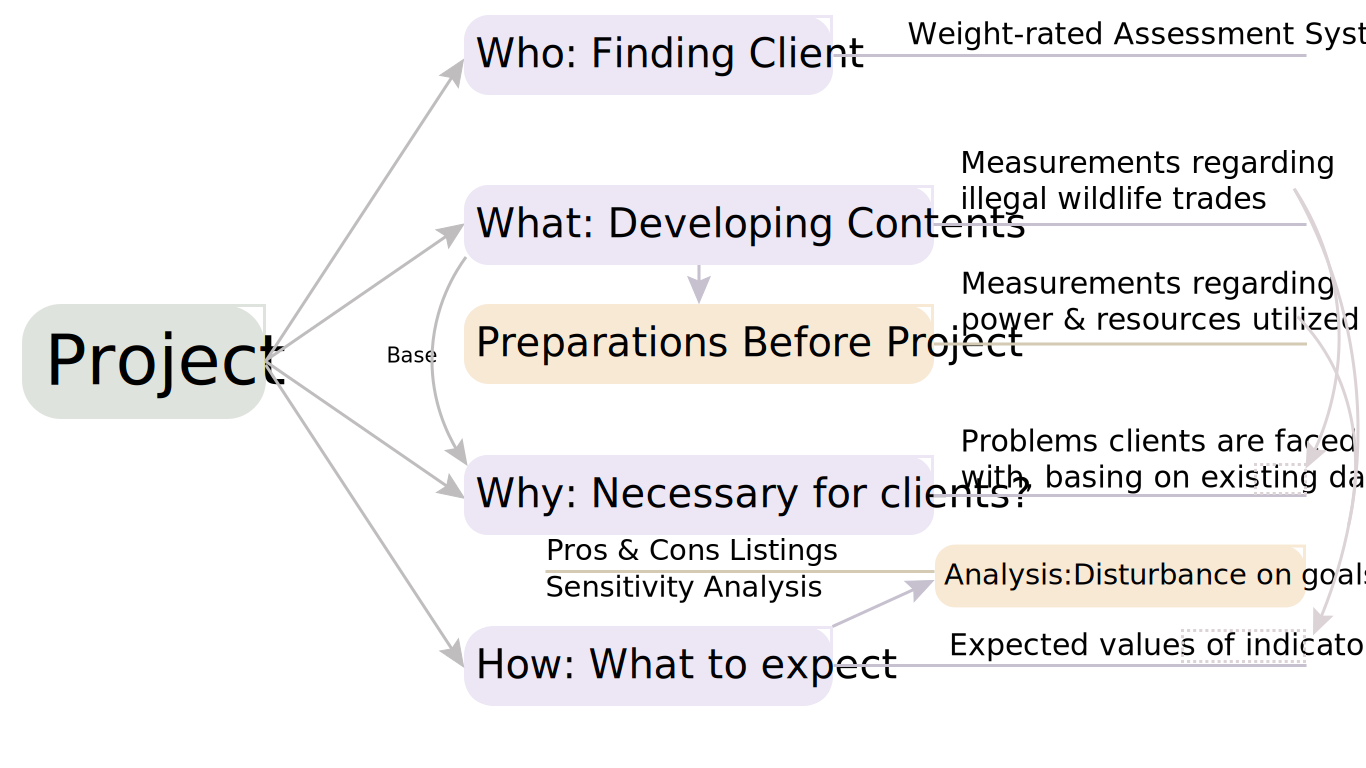
\includegraphics[width=.84\textwidth]{image16.png}
\end{figure*}

\clearpage
\section{Assumptions}
For the convenience when analysis turns under way, our team assumes that:
\begin{itemize}
	\item \textbf{All countries that feature high incomes are developed ones while those with lower salaries and wages are developing.} Our team holds the view that Gross Domestic Product (\textsc{gdp}) works when people attempt to tell the difference between both classes.
	\item \textbf{Weather will be fair and crop yield will be good in the next 5 years, dealing no damage to the normal livings of wildlife.} Probabilities of extreme climates and the catastrophes they bring about stay low up to now, and our project, therefore, need to make adjustments to adapt to the utmost occasions, should the worst things come along.
	\item \textbf{Civil riots will not take place on a global level in the next 5 years.} The conflicts are bound to spell the panics and pandemonium, sparing the illegal trades to grow wildly.
	\item \textbf{All data our team is accessible to are authentic and reliable.}
\end{itemize}
\section{Notations}
\begin{table}[htbp]
\centering
	\begin{tabular}{ll}
		\hline\hline
		Symbols & Definitions\\
		\hline
		$z_j$ & The performance of affairs against the illegal wildlife trades after the project launches\\
		$z_2$ & The extent to which clients have applied their power and resources as additions\\
		$z$ & The overall performance of affairs against the illegal wildlife trades\\
		$P$ &Possibility of realization for our team's project\\
		$x'_{ij}$ & Data of wildlife-related aspects in year $j$\\
		\hline\hline
	\end{tabular}
	\caption{Introduction to symbols of key parameters to be used and mentioned in this solution}
\end{table}
\clearpage
\section{Client Search}

\subsection{Factors Considered in Search of Clients \& Corresponding Parameters}
Our team is firmly convinced that potential clients along with factors that matters when searching for them can be categorized as follows.
\begin{figure}[htbp]
\centering

\includegraphics[width=0.8\textwidth]{image3.png}
\caption{Flow diagram illustrating the categories our team has reached}
\end{figure}

\begin{table}[htbp]
\begin{tabular}{||c|c|c||}
\hline
\hline
	Main Categories & Subcategories & Details\\
	\hline
	\multirow{9}{*}{Background ($A_1$)} & \multirow{3}{*}{Finance} & Costs taken for protection in favor of wildlife and habitats ($B_1$)\\
	
	&&Costs taken for environmental governance ($B_2$)\\
	&&Costs taken for blocks against traffic in wildlife ($B_3$)\\
	\cline{2-3}
	&\multirow{3}{*}{Influence}&Sphere of the client's influence ($B_4$)\\
	&&Relevant propagandas the client has done ($B_5$)\\
	&&Legislative movements from the client ($B_6$)\\
	\cline{2-3}
	&\multirow{2}{*}{Conscience}&Acknowledgement regarding the illegal wildlife trade ($B_7$)\\
	&&Identification in the field of wildlife protection ($B_8$)\\
	\cline{2-3}
	&Talents & Professional individuals \& experts the client features ($B_9$)\\
	\hline
	\multicolumn{2}{||c|}{\multirow{2}{*}{Willingness ($A_2$)}} & Client's willingness for wildlife preservation ($B_{10}$)\\
	\multicolumn{2}{||c|}{}& Marketing atmosphere where the client stands ($B_{11}$)\\
	\hline
	\multicolumn{2}{||c|}{\multirow{2}{*}{Motivation \& Execution ($A_3$)}} & Whether the client is motivated by seduction of incomes ($B_{12}$) \\
	\multicolumn{2}{||c|}{}& Whether the client is motivated by calls of duties ($B_{13}$)\\
	\hline
	\hline
	\end{tabular}
	\caption{Factors our team admire as critical ones to conduct assessments on clients}
\end{table}
\subsection{Weighting Factors in Search of Ideal Clients}
Our team got inspired by a steelyard balance when giving weight to the factors mentioned above and has made analogies to figure out the importance of one factor when comparing it with another. Our team is also persuaded that values obtained via the virtual weighing machine can also be employed by the judgment matrix $A$ of Analytic Hierarchy Process (\textsc{ahp}).
\begin{figure}[htbp]
	\centering
	\subfigure[Movement of the steelyard pivot counts for weight check]{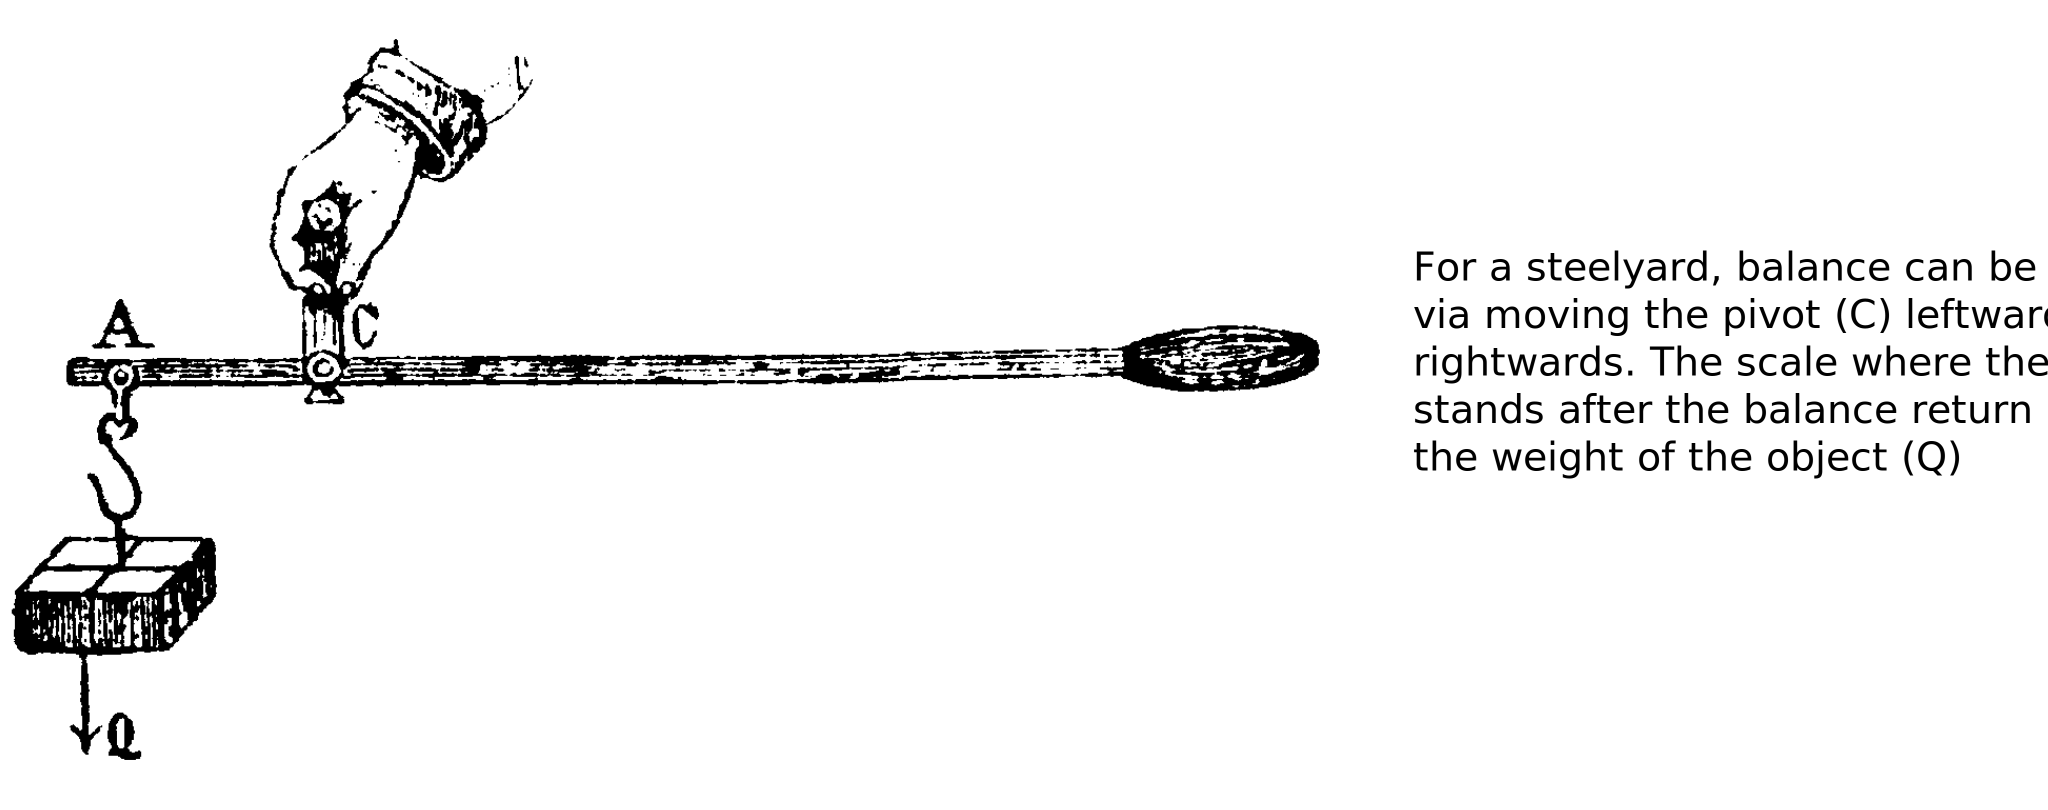
\includegraphics[width=0.75\textwidth]{image1.png}
	\label{Steelyard}}
	\subfigure[Our team's analogy for assessment between 2 factors]{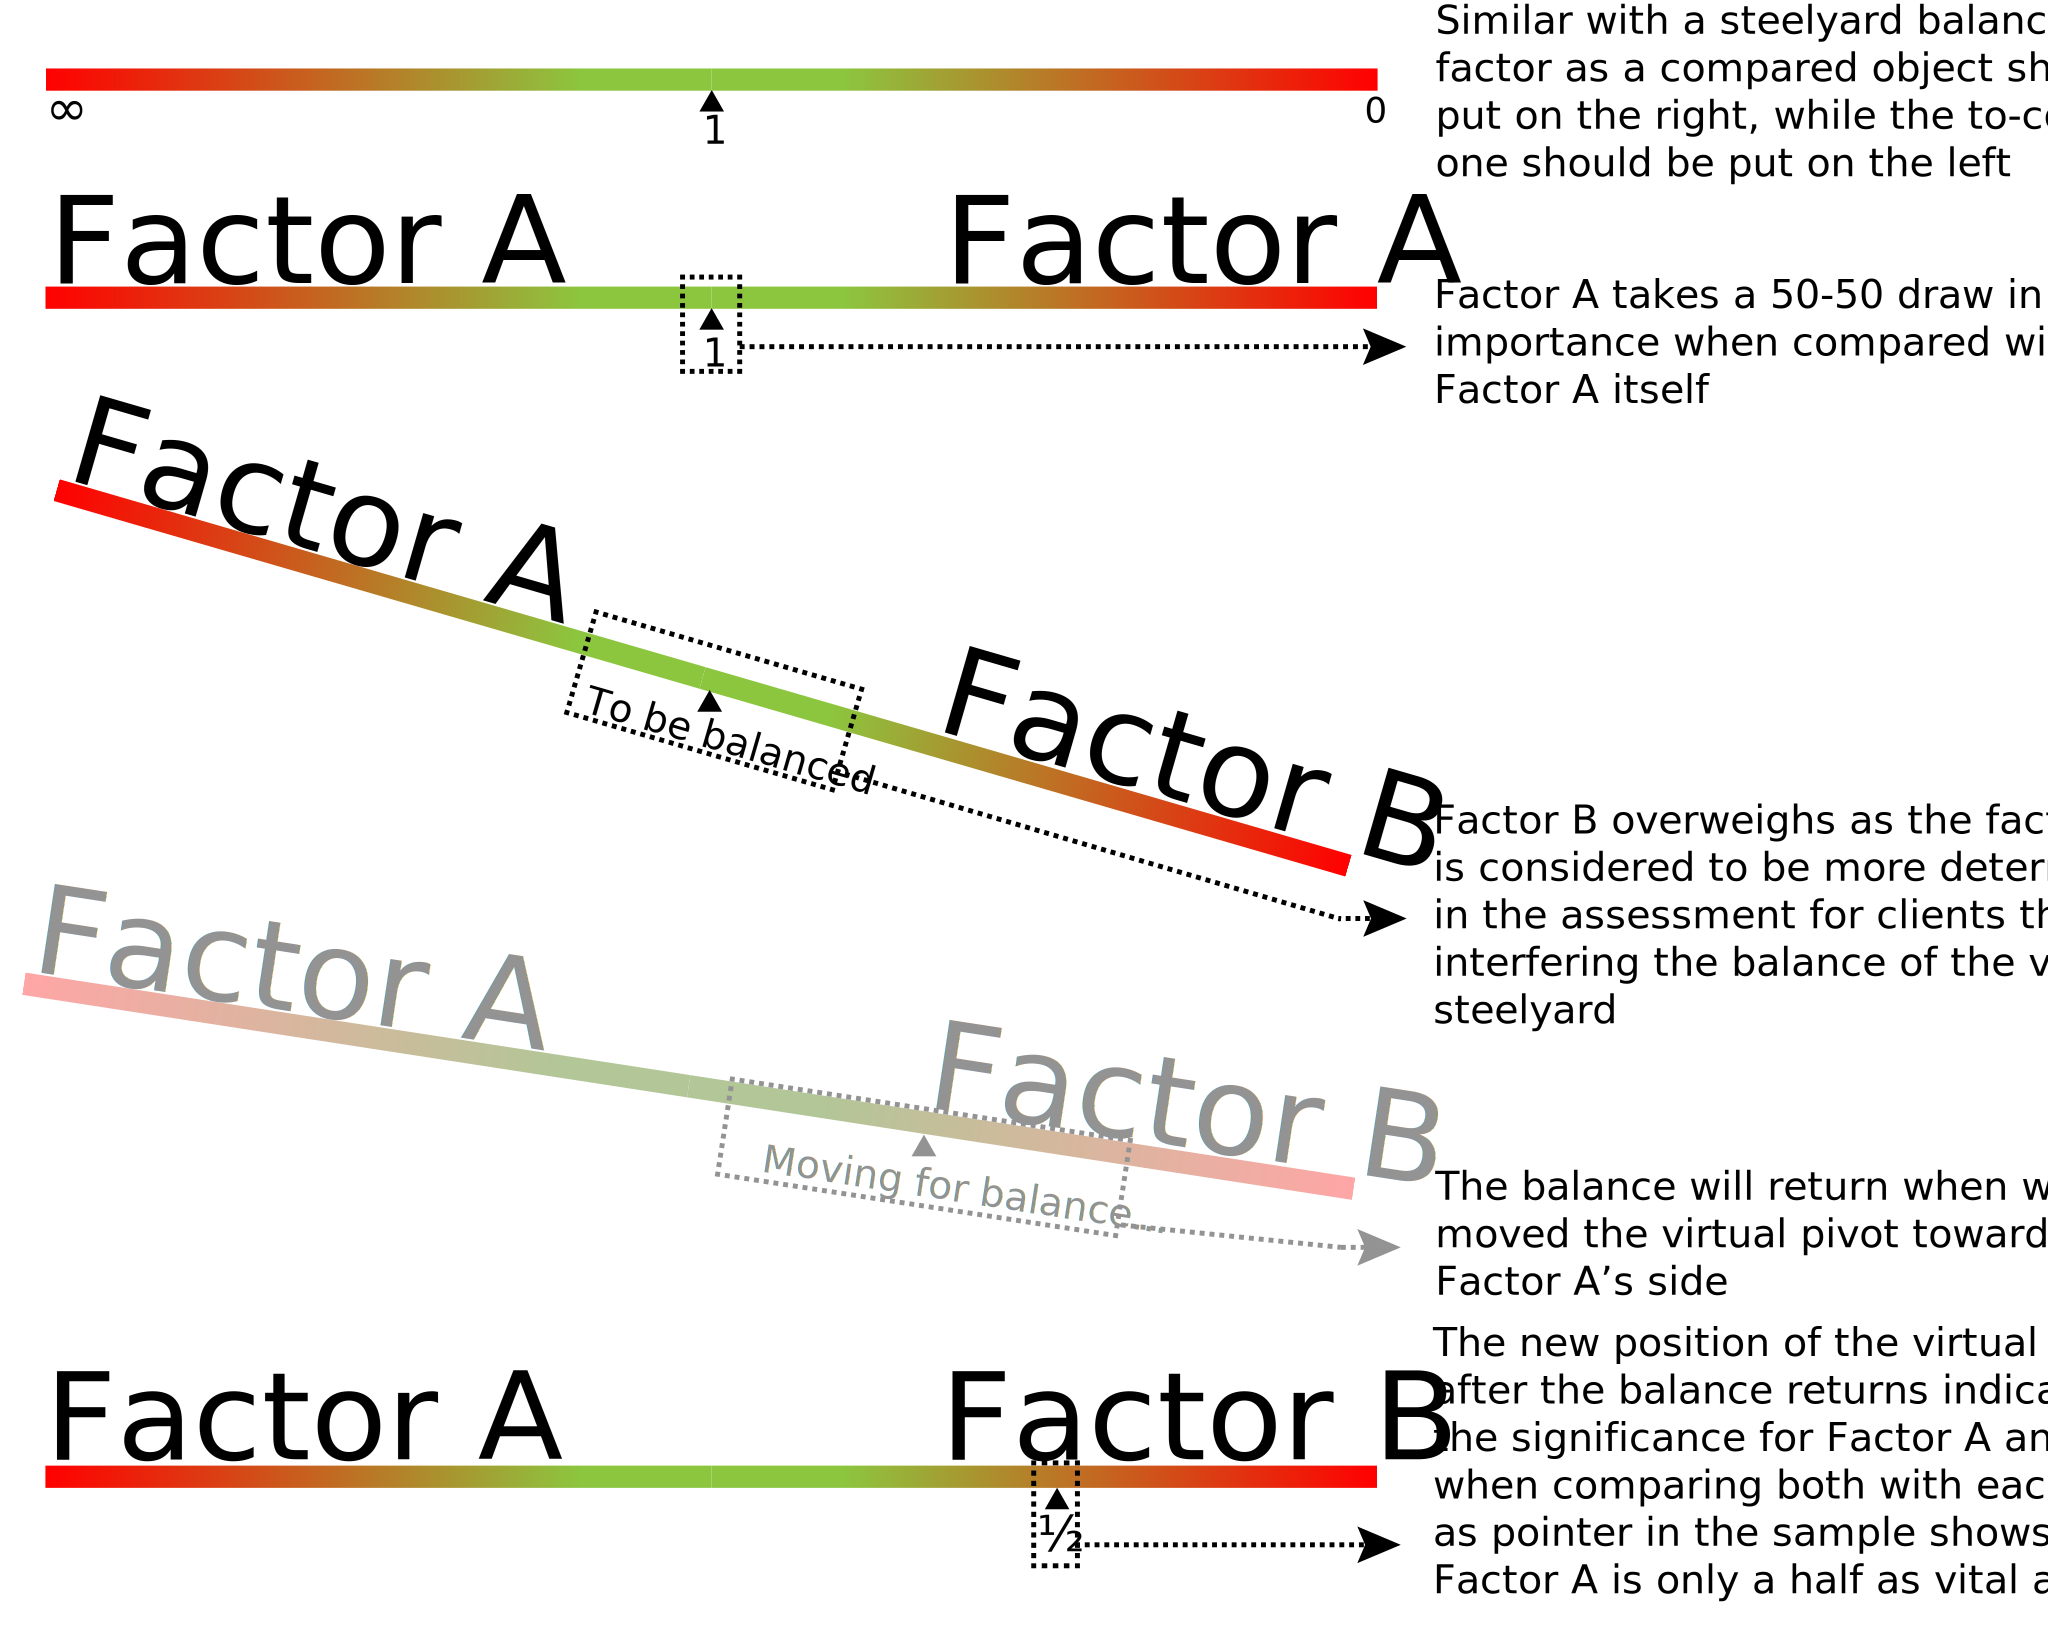
\includegraphics[width=0.75\textwidth]{image2.png}}
	\caption{Illustration for methods towards the score our team get when assessing a certain client}
	\label{Steelyard analysis}
\end{figure}

Discussions among 3 experts have it that the background of a client tops from all of the 3 main factors as the client's motivation bottoms, and the matrix can be reached as follows, where $A_{ij}$ stands for the importance of factor $A_j$ features when compared with factor $A_i$.

\begin{equation}
\begin{aligned}
	A&=\begin{pmatrix}
		A_{11} &A_{12} &A_{13}\\
		A_{21} &A_{22} &A_{23}\\
		A_{31} &A_{32} &A_{33}\\
	\end{pmatrix}
	\\&=\begin{pmatrix}
		1 &\frac{4}{11} &\frac{1}{11}\\
		\frac{11}{4} &1 &\frac{3}{7}\\
		11&\frac{7}{3}&1\\
	\end{pmatrix}
	\end{aligned}
\end{equation}

The maximum of eigenvalue $\lambda_{\max}$, in turn, can be reached that
\begin{equation*}
	\lambda_{\max}=3.03237,
\end{equation*}
and the consistency indicator (\textsc{ci}), along with the consistency ratio (\textsc{cr}) can be reached via the formula
\begin{equation}
	\begin{aligned}
		CI&=\frac{\lambda_{\max}-n}{n-1}\\
		&=\frac{3.03237-3}{3-1}=0.016185,
	\end{aligned}
\end{equation}
\begin{equation}
	\begin{aligned}
		CR&=\frac{CI}{RI}.
	\end{aligned}
\end{equation}
References have it that when the number of factors $n$ is 3, the random consistency indicator (\textsc{ri}) equals to 0.52, making \textsc{cr} able to be reached.
\begin{equation*}
	CR=\frac{CI}{RI}=0.03112.
\end{equation*}

%\begin{table}[htbp]
%	\centering
%	\begin{tabular}{c|ccc}
%		Factors ($A_i$) &$A_1$ &$A_2$ &$A_3$\\
%		\hline
%		Weights ($w_i$) &0.68&0.24&0.08\\
%	\end{tabular}
%	\caption{Weights our team has given to the 3 main factors for client assessment}
%\end{table}

\begin{wrapfigure}{r}{0.4\textwidth}
	\includegraphics[width=.4\textwidth]{image17-N.png}
	\caption{Pie chart of Weights of $A_1$, $A_2$ \& $A_3$ (inner ring) and the their sub-factors (outer ring)}
\end{wrapfigure}


Since the indicator features value that turns out below 0.1, the consistency of $A$ has been accepted by our team. Weights, afterwards, have been given by our team towards the 3 factors according to the matrix (see Figure 3).

For subcategories along with matching details, our team has put a rating system, where, for a single given indicator $B_k$, performances can be classified into 5 levels, into use. Experts also have assigned points for each of the level in pursuit of convenience to take place during calculations, the sample of which is shown in Table 3 next page.

\begin{figure*}[h]
\centering
	\includegraphics[width=0.9\textwidth]{image4.png}
	\setcounter{table}{2}
\end{figure*}

Ticks in different boxes implies the points $U_k$ the interviewee will get in the field of detail $B_k$. Our team then can work out the comprehensive score of one client via the formula
\begin{equation}
	Q=\frac{1}{9}w_1\sum_{i=1}^9U_i+\frac{1}{2}w_2\sum_{i=10}^{2}U_i+\frac{1}{2}\sum_{i=12}^{2}U_i,
\end{equation}
having applied weighted average.
\\ \\ \\
\subsection{Results \& Conclusion}
Scarcely had the experts finished the interview with the potential clients when our team cheetah-ed into the room to get the results. (The sheet shown in Table 3 is one of the used.) Our team discovered that points different potential clients have got are as shown in Table 4 after computations.

\begin{wraptable}{r}{0.5\textwidth}
\centering
\begin{tabular}{c|c}
	Categories & Scores (\textsc{pt})\\
	\hline
	Poor Governments & 61.74\\
	Rich Governments & 73.95\\
	Enterprises & 67.01\\
	For-Environment Organisations & 69.58\\
	For-Wildlife Organisations & 70.83
\end{tabular}
\setcounter{table}{3}
\caption{Scores of clients among categories}
\end{wraptable}

Our team is convinced by data that \textbf{governments with greater treasuries and wealth are the best choices for our team to turn to for help in order to utilize the project mentioned in this essay}. The conclusion does not go against our intuition, as offices that possess more funds are always more likely to set the personnels' views on extra fields. It is also rational that governors with higher incomes tend to be more positive when communicating with other bureaux to better laws and regulations. Affluent countries, where governments with high incomes are normally located, also proved to have a say on the international stage, making the project easier to spread.

Recent years have also read an increase in the number of reports that insinuate the impacts on wildlife traffic the broadening economic gap among poverty regions and well-off ones may have, as journalists also hinted the criticalness relevant policies from superpowers may present.$^{\cite{1}}$ The exposés themselves, hence, dispelled worries of our team on the prospective doubts and suspicions regarding the project to be given out along with its target clients from the public.

\section{Project Development: How It Cuts Down \& Why It Cuts Out}

\subsection{Project Introduction: How It Cuts Down Traffic of Wildlife}
To set the phased goal of the project, our team attempts to make predictions on trends of illegal wildlife trade in the next 5 years according to data published by the \textsc{u.s.}, an undoubtedly exemplary role of rich country, in the past.
\subsubsection{Pre-processing for Data}
Considering the possibilities that data last year have not been published up to the time when the paper is finished, our team decides to neglect numbers and percentages from 2023 which have been issued already. For statistics that turn out lost in the past years, our team equate them with the average of values under the same title one year later and earlier.
\begin{table}[htbp]
\centering
	\begin{tabular}{|c|c|c|c|}
		\hline
		Parameters & Definitions & Parameters & Definitions\\
		\hline
		\hline
		$i$ & Indicator for aspects &$i=1$ & Area of nature reserves \\
		\hline
		$i=2$ & Funds devoted for wildlife preservation& $i=3$ & Number of wildlife species \\
		\hline
		$i=4$ & Number of academic papers of wildlife & $i=5$ & Funds devoted for environment\\
		\hline
		$i=6$ & Area of wildlife habitats & $i=7$ & Vegetation Rate\\
		\hline
		$c_i$ & Weight of parameter $x_i$'s influence & $j$ & Year ($j\in [2013,2023], j\in \mathbb{Z}$)\\
		\hline
		$x_i$ & Array of data for indicator $i$ & $x'_i$ & Array $x_i$ after normalization\\
		\hline
		$x_{ij}$ & Data of $x_i$ in year $j$ & $x'_{ij}$ & Data of $x'_i$ in year $j$\\
		\hline
	\end{tabular}
\caption{Parameters \& corresponding definitions to be used in the pre-processing stage for data}
\end{table}
\begin{table}[htbp]
\centering
	\begin{tabular}{|c|c|c|}
		\hline
		Symbols & Definitions & Measurement \& Usage\\
		\hline\hline
		$a_i$ & \multirow{2}{*}{Constants to adjust the trends \& ranges of $x_i$} & \multirow{2}{*}{--}\\
		$b_i$ &&\\
		\hline
		$z_j$ & Indicator mirroring the severity of wildlife trade & The higher, the less serious\\
		\hline
	\end{tabular}
\caption{Definitions of indicators \& constants to be used in the pre-processing stage for data}
\end{table}

Since stats regarding the habitat coverage for wildlife are not on the list of annual updates, our team opts to make supplements thanks to \textbf{Assumption 2} and adds a few necessary disturbances.

Our team discovered that annual rate of changes in the wildlife habitat coverage stays low and that all data among fields feature large base, which may deny the overall correlativity between the habitat coverage and the number of species. Similar circumstances occur when we are analyzing the vegetation coverage. To dismiss the inherent denial, our team activates the normalization

\begin{equation}
	x'_{ij}=\frac{x_{ij}-\min(x_i)}{\max (x_i)-\min(x_i)}\
\end{equation}

to make the value of rates more noticeable. The normalization proves to be effective, as the inconspicuous spans have got greatly stretched by the mathematical lens (Figure 3 next page).

\begin{figure}[htbp]
\centering
	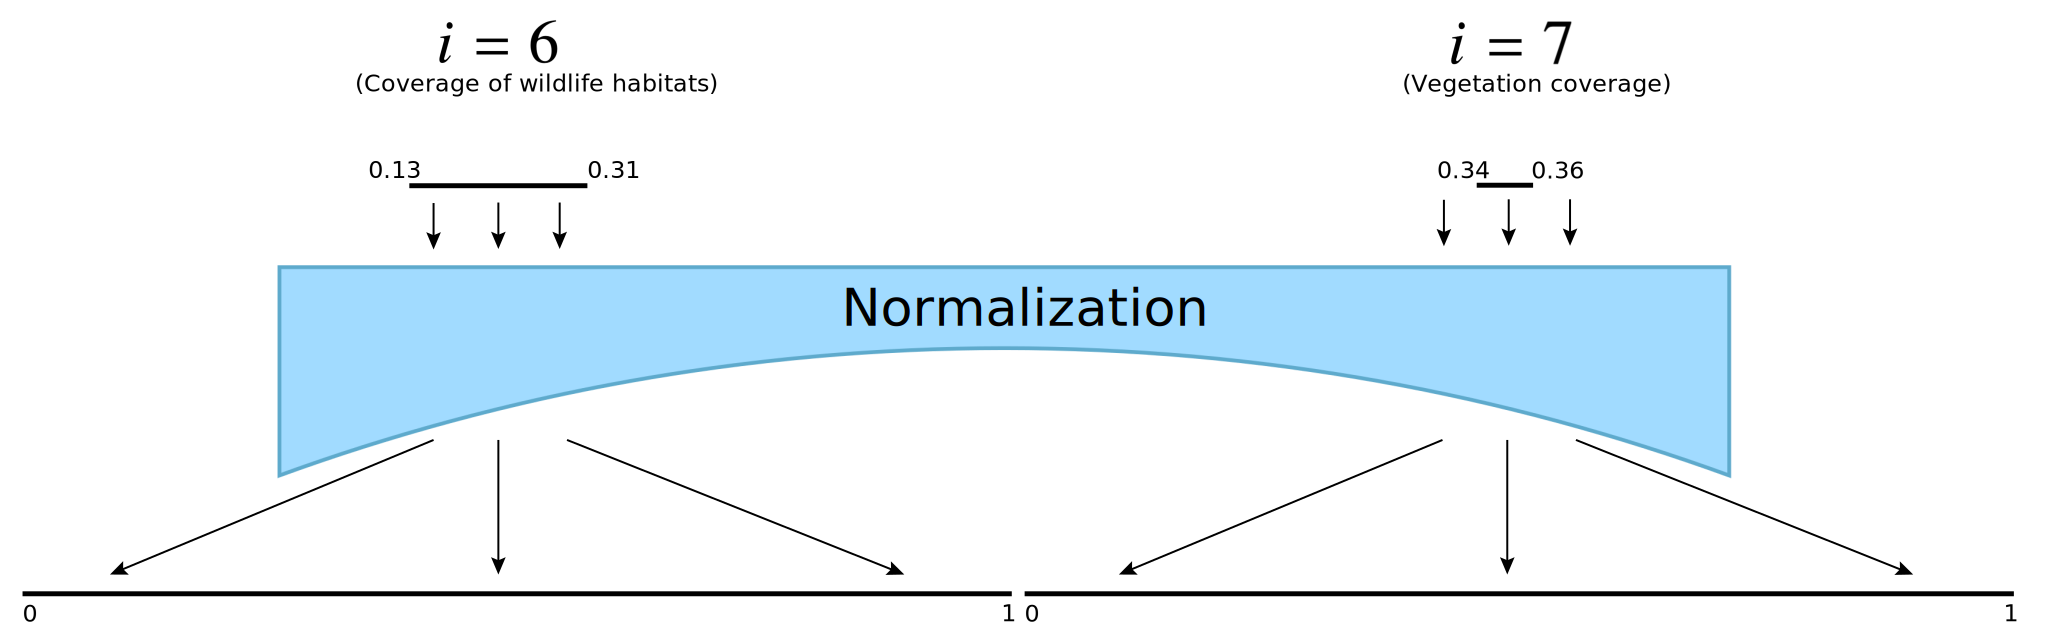
\includegraphics[width=0.6\textwidth]{image5.png}
	\caption{Ranges got greatly magnified owing to the concave lens composed of normalization}
\end{figure}

The processed data, along with those convenient enough for calculation upon the arrivals, will be used for analyses on their impacts respectively.

\subsubsection{Finding Steps towards the Reduction in the Wild Traffic}

Our team hold the view that when $i$ fluctuates to and from 5 and 7, the corresponding aspect may not make as much difference to the trade itself as the rest due to the strong fact that the effects they have are indirect. As a temporary result, our team decides to dive into swings of $x'_{1j}$, $x'_{2j}$, $x'_{3j}$ \& $x'_{4j}$.

It cannot be doubted that $x'_{ij}$ have been normalized into the range (0, 1). Our team, therefore, pick sine to analyze $x_{1j}$ \& $x_{4j}$. Meanwhile, quadratic functions are utilized to simulate the dynamic trend of impact that funds concerning wildlife have on the total result.

\begin{figure}[htbp]
\centering
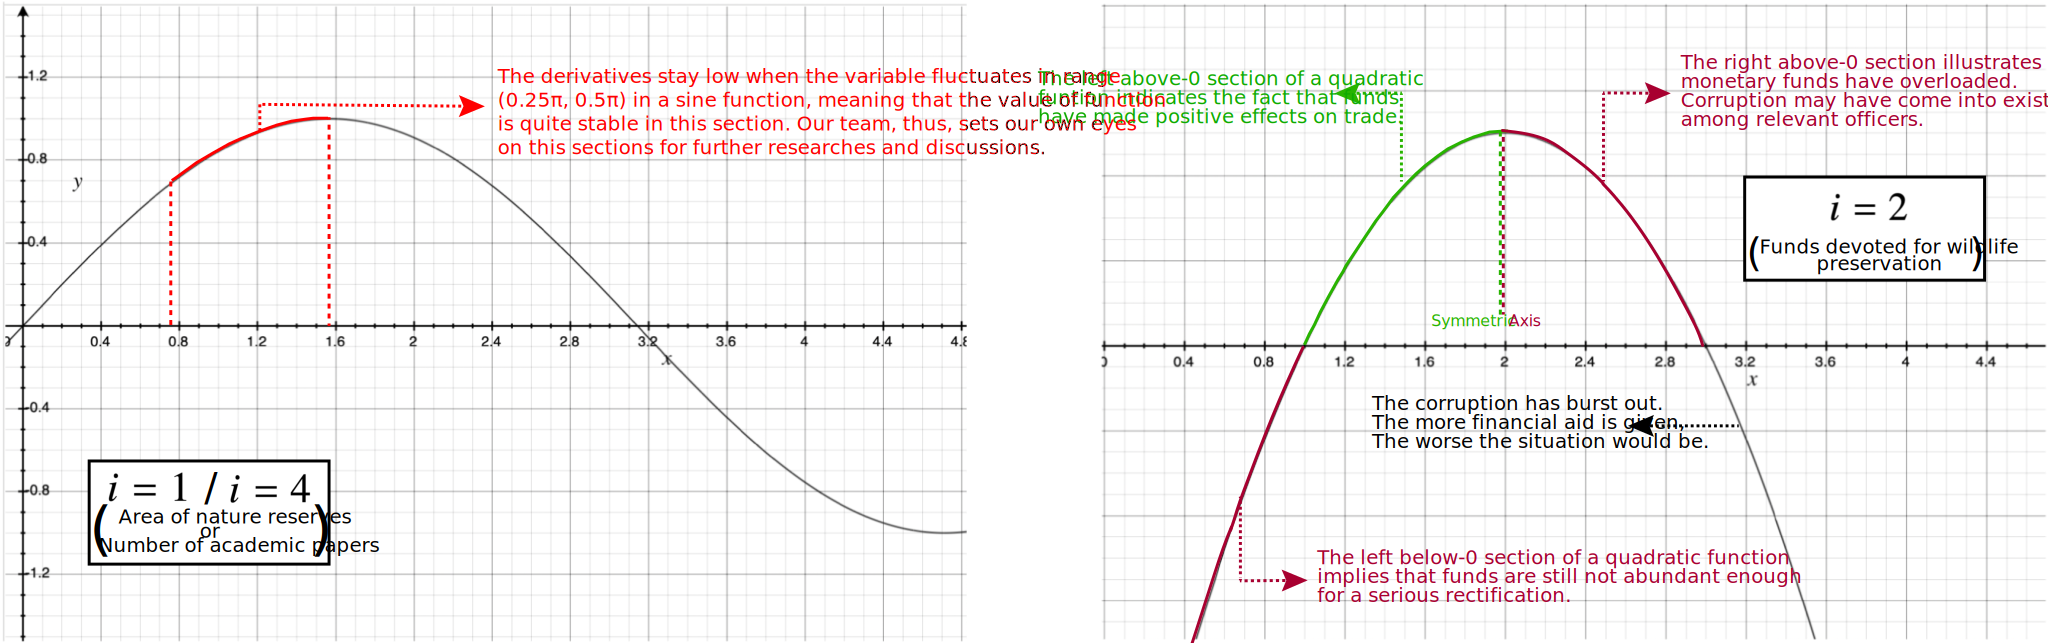
\includegraphics[width=\textwidth]{image6.png}
\caption{Illustrations of how our team reaches conclusion via graphs of functions}
\end{figure}

Our team also selects exponential functions to measure the trend of growth within the species of wildlife thanks to the function's practical meanings. As far as our team is concerned, changes in the number of species are best little birds that gesture the illegal traffic for wildlife.

In other words, measurements for the efforts conveyed by the client in a single year can be reached via the formula

\begin{equation}
	z_{j} = c_1 \sin(\frac{x'_{1j}+a_1}{b_1})+c_2(x'_{2j}+b_2)^2+c_3e^{a_3(x'_{3j}+b_3)}+c_4\sin (\frac{x'_{4j}+a_4}{b_4})+\sum_{i=5}^7c_i(x'_{ij}+a_i)^{b_i}+\gamma,
\end{equation}

where $\gamma$ is a constant specially designed for adjustments in indicators' range. Basing on the changing rate of $z_j$, our team as well as the client is able to make judgments on whether additions to $x_i$ in the year that comes up should be conducted.

\subsubsection{Results \& Conclusions for the United States}

After substituting the annual data which the \textsc{u.s.} issued from 2013 to 2023 into variables of Equation (6), our team yields values of the constants in the same equation.

\begin{table}[htbp]
\centering
	\begin{tabular}{c|cccccccccccc}
		Constants & $c_d$ & $c_2$ & $c_3$ & $c_t$ & $\gamma$ &$a_d$ & $a_3$ & $a_t$ & $b_d$ & $b_2$ & $b_3$ & $b_t$\\
		\hline
		Values & 0.65 & -0.3 & 3.56 & 0.48 & 4 & 5 & 0.34 & 1 & 6 & -1.7 & 1.87 & $\frac{1}{3}$
	\end{tabular}
\caption{Values of constants ($d\in\{1, 4\}, t\in\{5, 6, 7\}$)}
\end{table}

Hence the value $z_j$ can be obtained according to issued data year by year.
\begin{table}[htbp]
\centering
	\begin{tabular}{c|cccccccccc}
		$j$ & 2013 & 2014 & 2015 & 2016 & 2017 & 2018 & 2019 & 2020 & 2021 & 2022\\
		\hline
		$z_j$ & 3.0151 & 3.5031 & 4.3299 & 4.8021 & 5.7465 & 6.6909 & 7.1631 & 7.6353 & 8.1075 & 8.5997\\
	\end{tabular}
\caption{The performance of anti-trade affairs in the \textsc{u.s.} by year}
\end{table}

\begin{wrapfigure}{r}{0.29\textwidth}
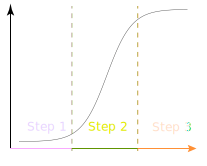
\includegraphics[width=0.29\textwidth]{image7.png}
\caption{3 steps of the anti-trade growth, subjective to the financial supports}
\end{wrapfigure}

The formula from Equation (6) can also reach an overall trend of growth regarding the anti-trade affairs that enjoys the rise of relevant financial aid. Our team divided the trend into 3 sections, according to the slope of the curve, as is illustrated in Figure 5. Fast rise depicted in Table 8 matches the second step, indicating the power of notes and coins the American government has spent. News concerning relevant involvements of the governors prove the conclusion as well as the correctness of our team's model.

To generalize, the formula in Equation (6) will be

\begin{equation}
	\begin{aligned}
		z_{j} = &0.65 \sin(\frac{x'_{1j}+5}{6})-0.3(x'_{2j}-1.7)^2+3.56e^{0.34(x'_{3j}+1.87)}\\
		&+0.65\sin (\frac{x'_{4j}+5}{6})+0.48\sum_{i=5}^7(x'_{ij}+1)^{\frac{1}{3}}+4.
	\end{aligned}
	\setcounter{equation}{6}
\end{equation}

The project can be made to the fullest with this formula. By calculations in pursuit of the annual value of $z_j$ and comparisons between the growing trend and the graph, the client and our team can discover the exact extent to which the funds have been injected. Adjustments and re-layout can be made accordingly, as funds are still required if the growth remains rapid and need to pause when fluctuations are not significant as expected. Specifically, policymakers can make minor modifications to investments in a certain field by comparing the trend with graphs of a simple function like quadratic functions and sine ones.

\subsubsection{Details of Project Scheme: Periodical Goals \& Correspondent Moves}

Our team set phased goals for the 5-year project according to the base-on-graph (Figure 5) predictions and have created instructions on steps to achieve them specifically. For the convenience when policymakers are analyzing the overall growth, our team has introduced new parameters for computations, analogizing what our team has done already during the pre-processing stage.

\begin{table}
	\begin{tabular}{cccc}
	\hline
		Symbol &Name & Definition & Equation\\
		\hline
		$f$ & Future Year & The year number when the project is under way & $f\in\complement_{\mathbb{N}_{2024}}\mathbb{N}_{2029}$\\
		\hline
		$x_{i,f}$ & Future Data & The data of $x_i$ in year $f$ & --\\
		\hline
		\multirow{5}{*}{$x''_{i,f}$} &  & Ratio of the difference between $x_{i,f}$ &\multirow{5}{*}{$x''_{ij}=\frac{x_{i,f}-\min(x_i)}{\max(x_i)-\min(x_i)}$}\\
		&Fake-&and minimum of existing data $x_i$ in the past decade\\
		&Normalized&to the difference between the minimum of $x_i$\\
		&Value&and the maximum of $x_i$\\
		&&($x_i$ is only an array of existing data in the past decade)\\
		\hline
	\end{tabular}
\caption{Definitions to symbols used in the project}
\end{table}

Our group marks it the ultimate that \textbf{normalized indicators for area coverage of nature reserve, funds for wildlife preservation and number of wildlife-related academic outcomes are supposed to be positioned on the steady section on the sine or quadratic functions}. Therefore, our team has set ideal values for $x''_{1,2029}$ \& $x''_{4,2029}$, and attempts to minimize the costs but maximize the performance has made the ideal $x''_{2, 2029}$ lowered.

Considering the fact that exponential functions applied to depict the trend of the number of species remain increasing and never converge, our team switches the horizons towards the maximum load of a ecological system along with the optimal size of a wildlife-friendly system and comes to the stats 1 to 2 centuries ago for references. Wildlife beings got widely over-hunted from late 19th century to mid 20th century throughout the planet, forcing our team to take data before the 1880s into concerns. The booming of technologies, industrialization and other double-edged catalysts towards both the methods of headcount and the ones that worsen the environment stimulate our team to set ideal value of $x''_{3,2029}$, $x''_{5,2029}$, $x''_{6,2029}$ and $x''_{7, 2029}$.

To chase after the ideal values, our team divides the period of 5 years into 2 steps, as anti-trade affairs may gain widespread and positive response in the first 3 years thanks to the coppered blooms on multiple aspects. The last year of the project may feature a quite slow rise, indicating the trend that assignments of the governors have come to the final phase. The 4th year is intentionally left blank for tactical change, as decision-makers can modify their strategies and investments according to the data and our team's model when the project is reported to have reached its midway.

In convenience of judgments on whether the clients have passed the mid-distance stone, our team also offers values for references in different fields. When values in annual reports exceed the ideal ones, the project has bypassed the mid-range point.

\begin{table}[htbp]
\centering
	\begin{tabular}{c|ccccccc}
		$i$ & 1 & 2 & 3 & 4 & 5 & 6 & 7\\
		\hline
		$x''_{i,mw}$ & 1.72 & 1 & 1.54 & 1.72 & 1.74 & 1.96 & 0.98\\
		$x''_{i,2029}$ & 1.96 &1.12 & 1.95 & 1.96 & 2.06 & 2.28 & 1.12\\
	\end{tabular}
\caption{Ideal fake-normalized values of $x''_i$ the indicator during ($x''_{i,mw}$) \& after ($x''_{i,2029}$) the project}
\end{table}

Adjustments can take place in the overall layout by decision-makers' extrapolations back to the original data, according to values of expected results along with existing data in the past decade.

\subsection{Project Flash-Back: Why It's Cut Out for the Client}


As is additionally shown in the overview of Figure 5, the atmosphere unfriendly to wildlife will remain almost unchanged in the very beginning, but the air is to change when funds continue to be injected into the field and the situation is bound to witness a sharp twist. However, as the old saying goes, quantitative changes won't necessarily spell the qualitative ones -- corruptions that the excessive capital injections give birth to, along with the possibilities that wildlife trades would have been nearly eradicated, lead to the saturated stage where the influence the funds have on the free scent that flora and fauna have been enjoying already hangs low. In normal conditions, the initial step is a sinkhole that traps the majority of low-income nations, as the governors have cost an arm and a leg but get few outcomes. For the clients we set our eyes on, nevertheless, our team is convinced that \textbf{savings of the government from rich countries can push the project towards the boundary of the last 2 stages without difficulties in the period of 5 years, as soon as they are not settled with current conditions and get determined to turn the tide.}

Our team is also confident that the project is attracting to the governors in that \textbf{the project can be divided into 3 steps and there is no need to do everything in one single step.} Also, it has been a proved-by-data cliché that rich countries dominate the list of destinations for luxuries that feature ivories and fur from wild beings$^{\cite{2}}$ as well as the fresh ingredients, $^{\cite{3}}$ (see Figure 7 next page) making the lie from the personnels that illegal wildlife trade has faded from the territories already self-defeating. \textbf{Pressure from both external facts and enforceability of the project itself may force the officers to sign on the documents concerning the specific entrance of the scheme.} Moreover, the trend can be easily captured in that samples of the \textsc{u.s.} in \textit{Step 2} features an average growth of over 0.7 per year and the value in \textit{Step 3} may feature no more than a fifth, \textbf{enabling governors to make decisions as soon as possible even when they are not accompanied by mathematic experts.}

\begin{wraptable}{r}{0.39\textwidth}
	\centering
	\begin{tabular}{ccc}
		\hline
		$j$&$x'_{7j}$&Change\\
		\hline
		2013 & 0.3465 & \textcolor[rgb]{0.6,0.6,0.6}{/}\\
		2014 & 0.3518 & \textcolor[rgb]{0.1,0.6,0.1}{+}\\
		2015 & 0.3602 & \textcolor[rgb]{0.1,0.6,0.1}{+}\\
		2016 & 0.3621 & \textcolor[rgb]{0.1,0.6,0.1}{+}\\
		2017 & 0.3489 & \textcolor{red}{-}\\
		2018 & 0.3573 & \textcolor[rgb]{0.1,0.6,0.1}{+}\\
		2019 & 0.3497 & \textcolor{red}{-}\\
		2020 & 0.3393 & \textcolor{red}{-}\\
		2021 & 0.3546 & \textcolor[rgb]{0.1,0.6,0.1}{+}\\
		2022 & 0.3585 & \textcolor[rgb]{0.1,0.6,0.1}{+}\\
		2023 & 0.3522 & \textcolor{red}{-}\\
		\hline
	\end{tabular}
\caption{Hesitation of policymakers (taking changes in $x'_{7j}$ as example)}
\end{wraptable}
Our team also noticed during analyses on parameters after pre-processing stage that some of them feature values that fluctuate erratically, which implies probabilities that the policymakers in the \textsc{u.s.} are aimless when adjusting backings on these fields. The world-largest nation is still suffering from the undirectedness, let alone governors from other rich countries. \textbf{Our project stands out on this occasion to offer instructions for investments on a single field, as supervisors can keep an eye on the growth curve of a separate aspect.} The formula is essentially a sum of impacts on all aspects -- by comparing the results of aspects and the trend of the function respectively, the layout of funds and decisions can be optimally adjusted.

Having taken all above into account, there is no reason for the governors to reject the carry-out of the project. \textbf{The project is easy to understand and operate, and turns out within the economic reach of a rich government. It also offers chances for instructive suggestions on investments in a certain field, as long as the field is mentioned in the declaration in the pre-processing stage.}

\begin{figure}[htbp]
	\centering
\subfigure[Heatmap of illegal wildlife imports worldwide (Deals)]{\includegraphics[width=0.49\textwidth]{image10.png}
	\label{Import heatmap}}
	\subfigure[Heatmap of illegal wildlife exports worldwide (Deals)]{\includegraphics[width=0.49\textwidth]{image9.png}}
	\caption{Heatmaps of illegal wildlife throughput worldwide (Processed from source: \cite{3})}
\end{figure}

\section{Project Extensions: Before \& After the Implementation}

\subsection{Wind-up: Preparations Before the Departure}

The project itself is just a tool to reduce the pressure and boost the comprehensive efficiency against the wildlife traffic. It could hardly reach the ceiling of profits, should the client be not as powerful as rated. Auxiliary capabilities along with preparations, therefore, are listed as demands as well before the implementations.
\subsubsection{Assumptions as Roadbeds}

Experts have made following assumptions for the sake of convenience when showing their requirements to the clients.

\begin{itemize}
	\item \textbf{Officers will not embezzle banknotes and cheques that are not listed in budgets of our project.} The assumption does not necessarily indicates the stink on a hog that officers will not sneak up on budget lists.
	\item \textbf{Qualities of talents who stand within a nation's reach as bonus employees in a certain period remain similar and the geniuses are all well-taught to be identical with wildlife.}
	\item \textbf{Likeliness do occur where residents and senior leaders globewide can reach a consensus on bans against the wildlife trade and will not quit after signing on the protocol.} Nonetheless, signatory countries or regions are allowed to do otherwise on specific occasions like wars or natural disasters.
\end{itemize}

Basing on the assumptions above, the paver named as \textit{Prior Demand} is about to start its engine.
\clearpage
\subsubsection{Requirements as Paving Stones}
Experts hold the view that basing on the assumptions above, arrangements before the policymakers take the project into effect can be listed as follows:
\begin{itemize}
	\item \textbf{Raise sufficient funds as backs for all kinds of movements.} The funds are supposed to differ from budget itself and should be protected from embezzlement, which has been vaccinated by \textbf{Assumption 1}.
	\item \textbf{Targeted talent reinforcement should step up.} State-owned offices lack supports from volunteers despite the fact that they are more likely to feature abundant talents for academic and scientific research, while World Wide Fund for Nature (\textsc{wwf}), the world-famous organization, goes to another extreme. To make it worse, situations have it that workers in the departments tend to be more utilitarian and lack practical experiences. Governors as clients, hence, are supposed to improve the intrinsic appearance by updating the Yellow Book with contacts of employees possessing wildlife-friendly spirits, as \textbf{Assumption 2} in the section ensures the quality of the newly hired on this aspect.
	\item \textbf{Legislative collaborations should be reached across territories.} It is widely consented that illegal wildlife trades are often conducted on an international stage, so improvements for laws are supposed to be high on the agenda before the project comes out. International communications can be reached to boost the formulation of relevant international treaties, basing on \textbf{Assumption 3} in the section. International alliance may indirectly make our project spread further as well, which anyway is not the major aim of this piece of guidance.
	\item \textbf{Clients, as representatives of the highest power of the state, should take an active role in pushing cooperations with institutes and colleges forward.} Tracks and monitoring works regarding the movements of wildlife, along with the climate where the creatures are located, can be facilitated by gadgets and utilities built by the researchers. Bonuses are rational to be given to universities and institutes that actively supply relevant alarms and offer equipments that benefits for the preservation.
	\item \textbf{Propaganda methods ought to be adjusted.} Advertisements have been everywhere asking citizens not to order dishes that features wildlife species listed on \textsc{iucn} red lists, and journals have pointed out the potential hazards and virus wildlife may bring to us human beings after intake for several times, $^{\cite{4}}$ but it just remains nearly unchanged. The decision-makers are supposed to draft on novel concepts so as to deeply move the masses to get rid of the illegal trade, adopting promoting approaches including social media or other digital resources.
\end{itemize}

To maximize the efficiency, our group attempts to establish a pareto multi objective optimization model in search of optimized solution in order to reduce these beforehand costs to the least but lift the positive returns to the most.

\clearpage

\begin{table}[htbp]
\centering
	\begin{tabular}{|c|c|c|c|}
			\hline
			Indicators & Definitions & Indicators & Definitions\\
			\hline
			\multirow{2}{*}{$z_1$} & Total costs for acquirements & \multirow{2}{*}{$z_2$} & Performance of fights\\
			& regarding extra power \& resources && against wildlife trades\\
			\hline
			$i$ & Aspects of preparations & $i=1$ & Funds\\
			\hline
			$i=2$ & Talents & $i=3$ & Legislative collaborations \\
			\hline
			$i=4$ & Scientific collaborations &$i=5$ &Propaganda\\
			\hline
			\multirow{2}{*}{$f(n_i)$}& An increasing function &$n_i$& Number of units used on aspect $i$\\
			\cline{3-4}
			&with declining derivatives&$\beta_i$ & Maximum of available power on field $i$\\
			\hline
			$\alpha_i$ & Cost for a single unit (constant) & \multicolumn{2}{c|}{( $0\leq\alpha_ip_i\leq\beta_i$ )}\\
			\hline
	\end{tabular}
	\caption{Indicators used in the pareto multi objective optimization model}
\end{table}
Equations can therefore easily reached that
\begin{equation}
	\min z_1=\sum_{i=1}^5\alpha _i n_i,
\end{equation}
and our team quantifies the returns of the preparations via the equation
\begin{equation}
	\max z_2=\sum_{i=1}^5f(n_i)
\end{equation}

to make measurements on the extent to which the client has utilized the ancillary controls.

Only when the paver has gone off-road can vehicles loaded with our team's project run smoothly on the roadway.

\subsection{Whizz-by: Impacts After the Project's Transit}

Predictions regarding outcomes of a project have been a repertoire already. However, the fact is that commonly-used models like \textsc{arima} and neuronal networks are only keys to large amount of samples but troublemakers to problems with fewer, as deviations are bound to spring out if our team activated the models. Therefore, our teams have attempted to refer to the Grey Forecasting Model to care for data in the past decade. Stats as predictions for the 5 years that come up popped up after the substitutions of the normalized data into the model, with which the indicator $z_j$ can be obtained. The indicator will mirror the situation to take place in the future without the interference of our team's project (see Figure 8 next page).

Area coverages of vegetations, nature reserves and wildlife habitats will also get improved according to the efforts spelled by the project, as funds for environmental protection increase. Climate throughout the planet, along with the ecosystem, will also benefit a lot from the shifts, other than the realization of our major purpose where the drop in the number of deals regarding the wild creatures will take place.

Power and resources engaged in the preparations for the carry-out can be added to the comprehensive assessment on the benefits the project will bring about. The overall performance of the project $z$ can be obtained, ergo, via a simple formula

\begin{equation}
	z=z_j+z_2.
\end{equation}

The check-in of $z_2$, beyond doubts, leads to a further improvement to fists against the malfeasant (see Figure 9 next page).

\begin{figure}[htbp]
\centering
	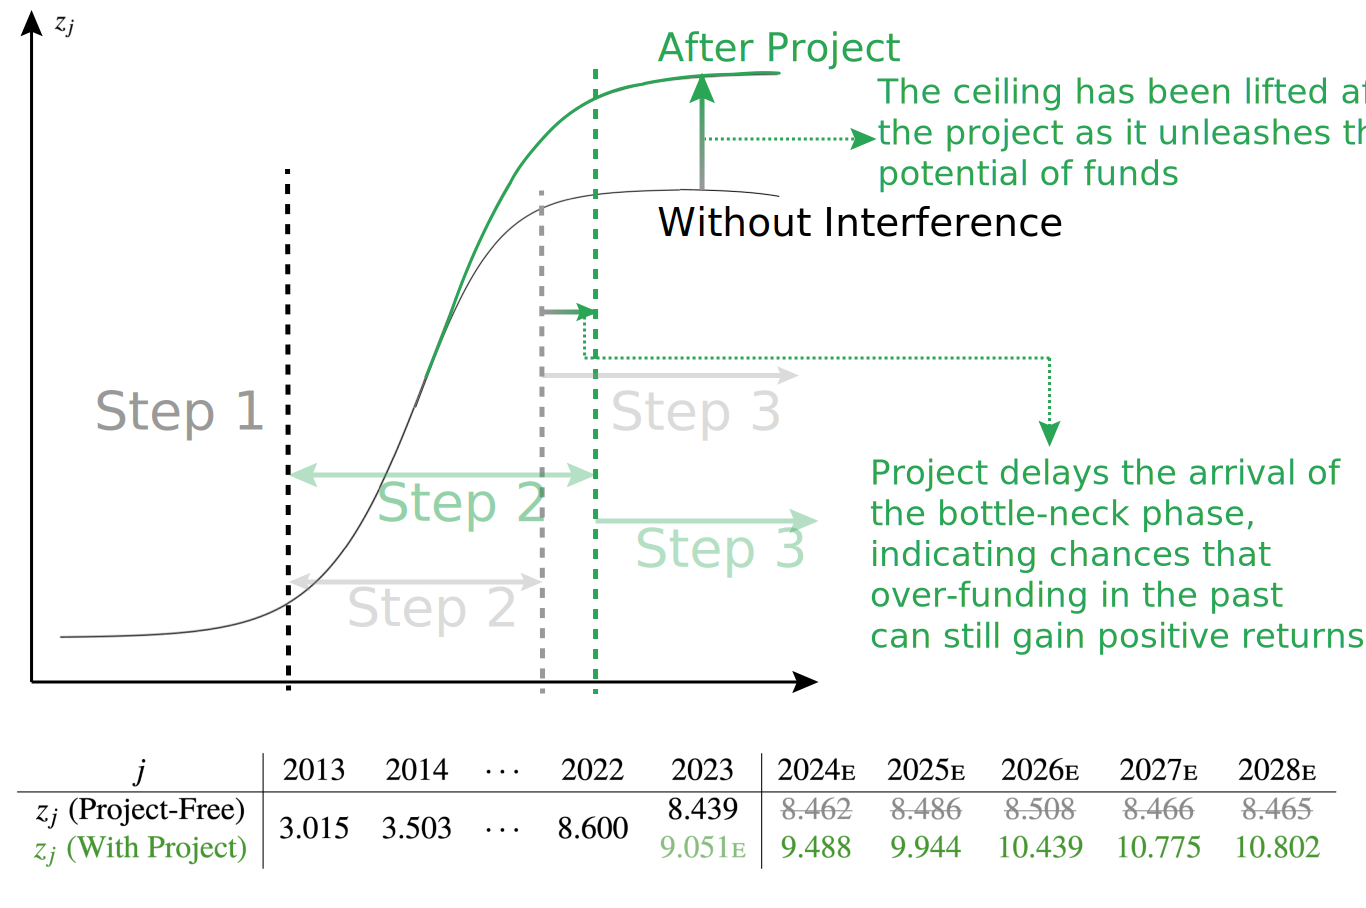
\includegraphics[width=0.8\textwidth]{image15.png}
	\caption{Illustrations of differences on $z_j$ that the project's arrival will make}
\end{figure}
\begin{figure}[htbp]
	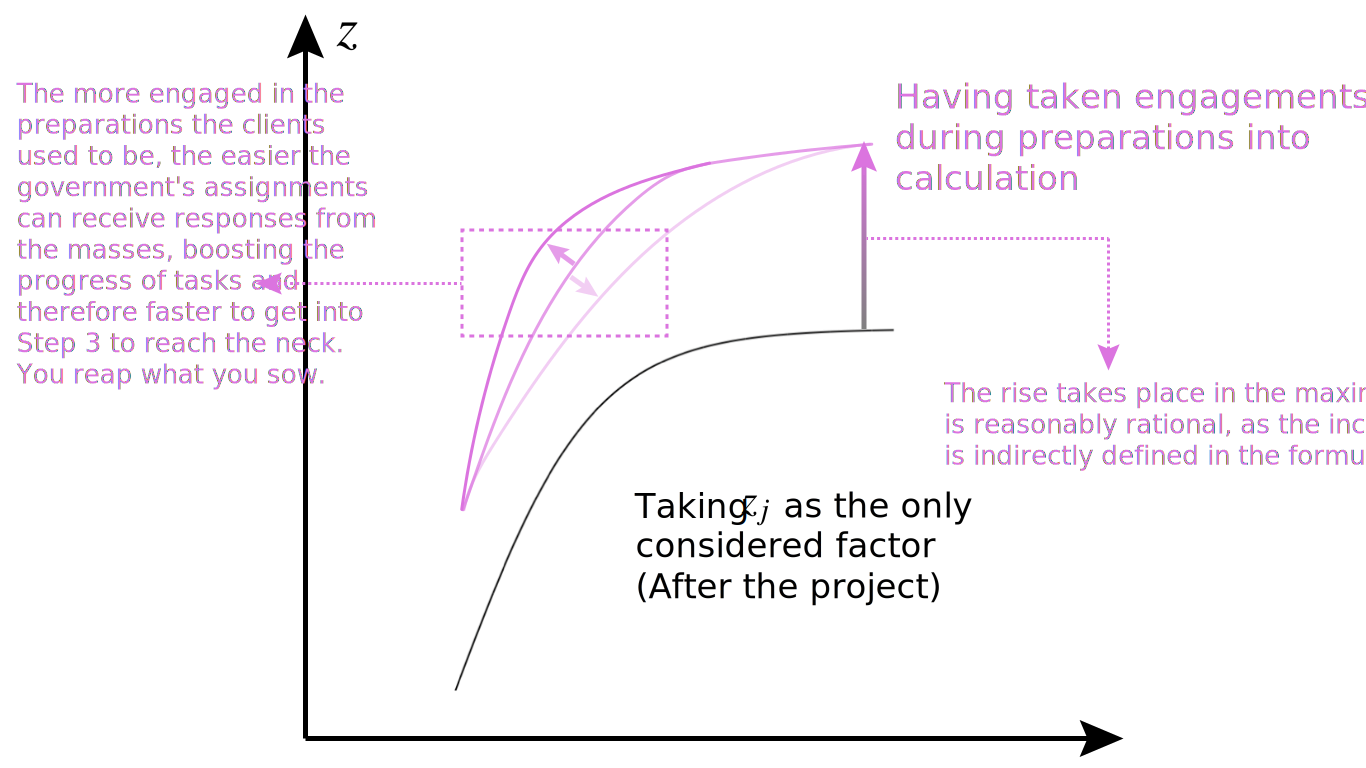
\includegraphics[width=0.8\textwidth]{image12.png}
	\caption{Illustrations of differences on $z$ after the additional consideration of $z_2$ on Step 2 \& 3}
\end{figure}
\clearpage

International collaborations are about to play a more vital role in supervisions concerning the illegal trades (see Figure 10), as it may help nations which are still suffering from low incomes and even poverty with preservations for wildlife from being hunted or turning freights. Laws and regulations that take effect worldwide can be taken as new strong barriers on the roadways to the trade in countries that shames on themselves thanks to lacks of relevant treaties that have made the cops turn blind eyes towards the transactions and therefore made the nations top the list regarding wildlife exports, as superpowers are supposed to shoulder the responsibilities to give a hand for the sake of sustainable development of the Earth. Live shares of information should be achieved to enhance the efficiency of law enforcements. Monitors tracking wildlife makes preventions for the creatures from being hunted real thanks to the rapid development of science and technology, and the skyrocket of relative bills may trigger further researches and higher employment rate, as the facilities need maintenance and updates.

\begin{figure}[htbp]
\centering
	\includegraphics[width=\textwidth]{image14.png}
	\caption{Overview of relationships among factors triggered by ecosystem improvements and international collaborations }
\end{figure}

To conclude, \textbf{the project proves to have strong and obvious positive impacts upon arrival, and the combinations of preparations and hard-hits make the most positive returns.} The illegal trade is not a simple piece of affair that has nothing to do with other fields, but requires groups and nations of all backgrounds to make joint efforts. Only through the concerted efforts of all sectors of society can such unwarranted businesses be significantly eradicated.
\clearpage
\section{Discussions}
What our team concentrates on is the likeliness for our project to reach the anticipated goal. Conditions and events are also of high possibility to behave like an ambush and conduct discovered attacks to affect the project's capabilities. As insurance for the smooth run of the mathematical beast shaped by the project, our team dives into models to scan the mines on the ground and give suggestions to avoid explosive ones when the eyeless beast is on the move.
\subsection{Possibilities of Goal-achieving}
Obstructions are inevitable before and after the launch of any movements, and the project our team has developed is not an exception. Wildlife trafficking, as a matter of fact, features astronomical-value transactions and are normally conducted in places beyond the reach of administrators.

Our team marks the number of obstructions on the list as $r$ and the probabilities a single obstruction ($q_i$) come to existence as $P(q_i)$, and the possibilities for our project to reach the goal ($P$) can be taken as hopes where the obstructions won't take place, which means
\begin{equation}
	P=\prod_{i=1}^r(1-P(q_i)).
\end{equation}
The obstructions vary, as corruptions or threatenings never fade away to the investigators and difficulties of undercover works keep existing. The over-length of the detection time also makes our clients unwilling to waste their hours on the bottomless maw. Conservation may occur on the phase of international collaboration, and conventions may pull the public from changing their stereotypes.

\subsection{Sensitivity Analysis}

The final results will deviate from the expected ones when parameters in models swing. The fluctuation can be caused by subjective judgments like attitudes of the experts who grade the clients and objective factors including current situations. Consequently, our team conducts the sensitivity analysis on models to decide on whether the models can stand the tests in the turbulence.

Our team fixes the focus on $c_i$, weights of different factors' influence on the anti-trade affairs for the analysis. The array of parameters experienced a thorough adjustment, where all the elements got changed by +10\%, +20\% and -10\%, and a componential one, where 2 of the elements increase by 5\% or 15\% and others remain unchanged, respectively. Our team compares the changed results with the expected ones mentioned in the project and discovered that swings will occur since $c_i$ as inputs change, but the overview of $z_j$'s trend will maintain (see Figure 11 next page). In other words, \textbf{relative relations will not alter and events that shatter the expectations of the project's outcomes or make the sequels streak do not exist}, proving the stability of our team's models.
\clearpage
\begin{figure}[htbp]
\centering
	\subfigure[Results of thorough adjustments]{\includegraphics[width=.45\textwidth]{image19-N.png}
	\label{Thorough results}}
	\subfigure[Results of componential adjustments]{\includegraphics[width=.45\textwidth]{image20-N.png}
	\label{Componential Results}}
\caption{Results of adjustments for sensitivity analysis}
\end{figure}
\subsection{Strengths \& Weaknesses}

On the basis of discussions within our team, pros and cons the models our team has built are featuring have been discovered and sorted below.

\subsubsection{Strengths}
\begin{itemize}
	\item The subjectivity of the model for assessment in search of clients seems to have declined as it employs fuzzy comprehensive assessment matrices to reduce the reliance on the \textsc{ahp} methods, making the model more objective and accurate.
	\item The model stars capabilities of generalization, as the \textsc{u.s.}, the sample according to which we develop our project, is a typical representative of high-income countries.
	\item Structures of our models are independent of each other, minimizing the impacts from one of them on another.
	\item Models our team have used are mostly inspired-by-real-gadgets or widely-used ones, making our models uncomplicated to be explained and more understandable.
\end{itemize}
\subsubsection{Weaknesses}
\begin{itemize}
	\item Arbitrary categorization occurred when judging the level of income of different countries worldwide, making the range of a single category oversize.
	\item The humble database denies our team from ensuring the high accuracy of the predictions, as the indicators and constants in models are directly affected by relevant data. Limitations, therefore, come to existence when our team attempts to fetch more indicators, as the number of closed cases have failed to help when quantitative analyses of models are under way.
	\item Lack of data declined our team from tests for models on extra resources and power during the wind-up stage.
\end{itemize}
\clearpage
\section{Memorandum to the Client}
\hrule\hrule\hrule
\text{}\\
\texttt{\text{ }\text{ }\text{ }DATE: 5 February, 2024}\\
\texttt{\text{ }\text{ }\text{ }\text{ }\text{ }TO: All Staff}\\
\texttt{\text{ }\text{ }\text{ }FROM: Team \#\Team, ICM Society}\\
\texttt{SUBJECT: Project Against Illegal Wildlife Trades In Brief}\\
\hrule
\text{}\\
\texttt{Please accept gratitudes from our team again for your trusts in our project a-}\\
\texttt{long with whole-hearted devotions to the affairs against illegal wildlife tra-}\\
\texttt{fficking. Our team is excited to leave a memo here as information \& guidance }\\
\texttt{in case you are faced with difficulties on concepts and usages of the project.}\\
\text{}\\
\texttt{The based-on-data project features top efficiency in reducing the unlawful wi-}\\
\texttt{ldlife transactions if employed with the help of combinations of detailed dat-}\\
\texttt{a, additional power \& extra resources. Taking it into account that deals on  }\\
\texttt{the creatures are normally finished outside the law, you don't have to clarify}\\
\texttt{the exact total numbers of contracts - the popularities of trades can be indi-}\\
\texttt{rectly mirrored by subtle changes that take place in the ecosystem, like numb-}\\
\texttt{er of species within the ecological chains that involves the treasures for bo-}\\
\texttt{unty hunters and area coverage of vegetations. Mathematical formula are esta-}\\
\texttt{blished as well to reflect the hardness of your fists when punching the lawbr-}\\
\texttt{eaking market, and please feel free to adjust the involved parameters accordi-}\\
\texttt{ng to your specific conditions.}\\
\text{}\\
\texttt{Our team also got a crush on the power and reach for resources when we signed}\\
\texttt{on the agreements, which defines you servants of the people in a superpower.}\\
\texttt{Our team, therefore, strongly recommend that you give full play to them on the international stage and take the lead in improving relative letters of laws }\\
\texttt{and treaties. Shifts on stereotypes of your electors regarding wildlife are}\\
\texttt{also supposed to be in your to-do lists, as cliché goes among economists that}\\
\texttt{where there is a call, there is a mall. You ought to step up with progress of}\\
\texttt{relative technologies, funds and cultivations for matching talents.}\\
\text{}\\
\texttt{It does not matter whether the magnets that pick you up are made up of copper}\\
\texttt{or conscience when anti-trade recruitment begins, it is your strong willingne-}\\
\texttt{ss in favor of wildlife preservation that tops you from all other applicants}\\
\texttt{for the project's appliance. Our team also appreciates it when you have done}\\
\texttt{a lot before the assessments, which has relieved more burdens on your shoulde-}\\
\texttt{rs than expected. So stay confident, and our team is looking forward to the }\\
\texttt{environmentally-friendly outcomes 5 years later.}\\
\text{}\\
\texttt{Wish you have a pleasant day.}\\
\texttt{Team \#\Team}
\\
\hrule\hrule\hrule
\clearpage
\begin{thebibliography}{99}
\addcontentsline{toc}{section}{References}
	\bibitem{1} "Gap between the rich countries and the poor drives the international wildlife trade". \textit{BBC news (Chinese)}. 2021-05-07.
	\bibitem{2} \texttt{https://www.traffic.org/site/assets/files/13112/uwa-traffic-cwt-2019-digest.pdf} (\textit{Counter Wildlife Trafficking Digest: South East Asia and China, 2019 -- Issue III}, \textsc{usaid} Wildlife Asia, 2020-09-03)
	\bibitem{3} \texttt{https://www.traffic.org/}
	\bibitem{4} "SARS may come from wildlife". \textit{Jiefang Daily}. 2003-05-25.
	\bibitem{5} Chen, J.; Chen, M.; Li, N. (2024). "Research on practical teaching evaluation of sand table simulation based on fuzzy analytic hierarchy process". \textit{Project Management Technology}, 22(01), 62-66. ISSN 1672-4313.
	\bibitem{6} Zimmerman, M. E. (2003). "The black market for wildlife: Combating transnational organized crime in the illegal wildlife trade". \textit{Vand. J. Transnat'l L.}, 36, 1657.
	\bibitem{7} Chen, J.; Hu, C.; Yang, F.; Deng, L. (2021). "Study on the Governance Strategy of Illegal Trade in Wildlife and Its Products". \textit{Issues of Forestry Economics}, 41(02), 136-145. doi:10.16832/j.cnki.1005-9709.20200280 . ISSN 1005-9709.
	\bibitem{8} Liang, Z.; Hu, J.; Hu, S.; Zhao, J.; et al. (2020). "Understanding and changing wildlife consumption behavior from a multidisciplinary perspective". \textit{Biodiversity Science}, 28(05), 606-620. ISSN 1005-0094.
	\bibitem{9} Peng, Sh.; Li, Q.; Ren, H. (2002). "Impact of Climate Change on Wildlife". \textit{Acta Ecologica Sinica}, (07), 1153-1159. ISSN 1000-0933.
\end{thebibliography}
\clearpage
\addcontentsline{toc}{section}{Appendix}
\appendix
\hiddensection {Codes for Heat Map Indicating Illegal Wildlife Deals Worldwide (Key Part)}
\lstset{ 
  backgroundcolor=\color{white},    
  basicstyle=\ttfamily,        
  breakatwhitespace=false,         
  breaklines=true,                 
  captionpos=b,                    
  commentstyle=\color{green},    
  deletekeywords={...},            
  escapeinside={\%*}{*)},          
  extendedchars=true,               
  frame=single,	                   
  keepspaces=true,                 
  keywordstyle=\color{blue},       
  language=Python,                 
  morekeywords={*,...},            
  numbers=left,                    
  numbersep=5pt,                   
  numberstyle=\tiny\color{gray}, 
  rulecolor=\color{black},
  showspaces=false,                
  showstringspaces=false,          
  showtabs=false,                  
  stepnumber=1,                    
  stringstyle=\color{orange},     
  tabsize=2,	                   
  title=\lstname                   
}
\begin{lstlisting}[language=Python]{illegalThroughput.py}
from pyecharts import options as opts
from pyecharts.charts import Map

value1 = [889795,413070,367272,145020,116706,81008,63073,53047,
	50432,44119,33597,32175,26219,20476,15232,15218,15146,14743,
	14336,13644]
country = ["United States","China","Canada","Germany","Italy","Turkey","Thailand","colombia","Viet Nam","Greece","South Africa","Singapore","France","United Kingdom","Portugal","Switzerland","Russian Federation","Norway","Mexico","Spain"]
c1 = (
    Map()
    .add(" ", [list(z) for z in zip(country, value1)], "world")
    .set_series_opts(label_opts=opts.LabelOpts(is_show=False))
    .set_global_opts(
        title_opts=opts.TitleOpts(title=" "),
        visualmap_opts=opts.VisualMapOpts(max_=900000),
    )
    .render("map_world.html")
)

value2 = [530973,443240,302153,267993,256072,166831,78201,68811,
	58676,54740,33164,27287,20373,16638,14402,14013,11333,11081,
	10547,8996]
country = ["Namibia","United States","Australia","Saint Kitts and Nevis","Canada","Peru","South Africa","Argentina","Zimbabwe","Russian Federation","Bangladesh","Indonesia","Gabon","United Republic of Tanzania","Democratic Republic of the Congo","Costa Rica","Madagascar","Senegal","Liberia","Mauritius"]
c2 = (
    Map()
    .add(" ", [list(z) for z in zip(country, value2)], "world")
    .set_series_opts(label_opts=opts.LabelOpts(is_show=False))
    .set_global_opts(
        title_opts=opts.TitleOpts(title=" "),
        visualmap_opts=opts.VisualMapOpts(max_=533000),
    )
    .render("map_world2.html")
)

\end{lstlisting}
\end{document}